\tikzstyle{input}=[draw,fill=red!50,circle,minimum size=10pt,inner sep=0pt]
\tikzstyle{hidden}=[draw,fill=green!50,circle,minimum size=10pt,inner sep=0pt]
\tikzstyle{output}=[draw,fill=blue!50,circle,minimum size=10pt,inner sep=0pt]
\tikzstyle{bias}=[draw,dashed,fill=gray!50,circle,minimum size=10pt,inner sep=0pt]

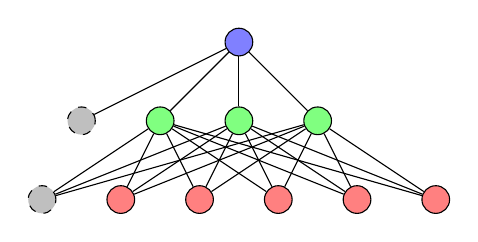
\begin{tikzpicture}
  \node (b1)[bias] at (-1,0) {};
  \node (b2)[bias] at (-0.5,1) {};
  \node (i1)[input] at (0,0) {};
  \node (i2)[input] at (1,0) {};
  \node (i3)[input] at (2,0) {};
  \node (i4)[input] at (3,0) {};
  \node (i5)[input] at (4,0) {};
  \node (h1)[hidden] at (0.5,1) {};
  \node (h2)[hidden] at (1.5,1) {};
  \node (h3)[hidden] at (2.5,1) {};
  \node (o1)[output] at (1.5,2) {};

    \draw (b2) -- (o1);
    \draw (h1) -- (o1);
    \draw (h2) -- (o1);
    \draw (h3) -- (o1);

    \foreach \j in {1, ..., 3}{
        \foreach \i in {1, ..., 5}{
            \draw (h\j) -- (i\i);
        }
        \draw (h\j) -- (b1);
    }
\end{tikzpicture}